\documentclass[11pt,a4paper]{article}
\usepackage[utf8]{inputenc}
\usepackage[T1]{fontenc}
\usepackage[english]{babel}
\usepackage[margin=2.1cm]{geometry}
\usepackage{booktabs,array,tabularx}
\usepackage{xcolor}
\usepackage{graphicx}
\usepackage{pgfplots}
\pgfplotsset{compat=1.17}
\PassOptionsToPackage{hyphens}{url}
\usepackage[hidelinks]{hyperref}
\usepackage{enumitem}
\setlist{nosep,leftmargin=1.4em}
\emergencystretch=3em

\definecolor{impl}{HTML}{3B6EA8}
\definecolor{rev}{HTML}{8FB3DA}

\title{Sweatshop on P-Chess: lane \texttt{core}, rework of PR \#10\\\large Corrupt stats files and a repertoire check skipped during the catalog load (HIST-001, OPEN-002, OPEN-004); GPT-6.1 Sol lineup}
\author{Foreman, session \texttt{sweatshop/core/2026-10-25-0159}}
\date{25 October 2026}

\begin{document}
\maketitle

\section*{Summary}

The independent review of session PR \href{https://github.com/Laginho/P-Chess/pull/10}{\#10} at
head \texttt{6fbac3e} (\texttt{gpt-6.1-sol xhigh}, run by the supervising session) returned
``do not merge'' with two blocking findings. The foreman reopened the three owner tickets on
the session (\texttt{24783fc}) and relaunched the same session at 11:01, \texttt{-Models 'stage
2 gpt-6.1-sol high, hard gpt-6.1-sol xhigh, stage 3 gpt-6.1-sol xhigh'}, pid 17404. The driver
ended at 11:43 with ``Nothing runnable''. This report continues
\path{2026-10-25-sweatshop-day-core.pdf}, which covers the run that built the ten tickets.

\begin{itemize}
  \item \textbf{Produced:} the three reopened tickets repaired test first, re-reviewed and
        merged again on the session: HIST-001, OPEN-002, OPEN-004, each with no new finding.
        PR \#10 still holds 10 tickets, all \texttt{Review: agent}, \texttt{Verdict: Approve}.
        Gate 241 passed, 0 failed (from 235).
  \item \textbf{Cost:} \textbf{\$4.10} at API list price over 6 stages:
        \texttt{gpt-6.1-sol xhigh} \$3.63 (\$1.55 as hard implementer, \$2.08 in review),
        \texttt{gpt-6.1-sol high} \$0.48. Codex quota: 3 points of the weekly window
        (\texttt{gpt-6.1-sol xhigh} 2, outside the stages 1, \texttt{gpt-6.1-sol high} 0).
  \item \textbf{What went wrong:} the three defects were present when each ticket was first
        approved; the ticket reviews did not try a hand-edited or partly written stats file,
        or a setting changed while the catalog loads. The session review caught them.
  \item \textbf{Provisional verdict:} a cheap, clean rework (\$1.37 per ticket, 11--15~min per
        ticket end to end). The lesson is for the ticket reviews: persisted files and
        settings changed during an \texttt{await} need a probe.
\end{itemize}

\section*{What was done}

\textbf{HIST-001}: a stats file that parses but holds a partial result record (only
\texttt{wins}) or a bare number no longer crashes the end of the game. The bad record counts as
zeros, every valid record is kept, and the result and review screens show a warning.
\path{core/history.gd}. Before, the game-end accounting raised a script error reading
\texttt{losses}, and the review opened as if nothing had happened.

\textbf{OPEN-002}: a practice count saved as text, or negative, is read as 0 and the other
counts are kept; Maia's book still picks its practice target, and the result screen shows the
same warning. \path{core/history.gd} (\texttt{practice\_counts}). Before, the book's target
selection raised a script error.

\textbf{OPEN-004}: turning on ``Check my moves against my repertoire'' while the opening catalog
is loading no longer starts a game with an empty repertoire. After the catalog load,
\path{ui/main.gd} decides again whether the repertoire is needed and, if its load failed,
returns to the setup screen with the error. Before, the decision was taken before the wait, and
the review then showed no repertoire badges.

\section*{Timeline}

\begin{tabularx}{\linewidth}{@{}lX@{}}
\toprule
10:55 & Supervisor relays the PR \#10 review (do not merge, 2 blocking). Foreman: owners from \texttt{git blame} (HIST-001 \texttt{7e5b8a4}, OPEN-002 \texttt{cf0419f}, OPEN-004 \texttt{cf5a29a}); tickets reopened with the findings, regressions and HIST-001's second-reopen diagnosis (\texttt{24783fc}). \\
11:01 & Relaunch, pid 17404, same session. \\
11:16 & HIST-001 (hard) merged again, 0 findings. \\
11:30 & OPEN-002 (hard) merged again, 0 findings. \\
11:42 & OPEN-004 merged again, 0 findings; ``Nothing runnable''. \\
\bottomrule
\end{tabularx}

\section*{Per stage}

{\small
\begin{tabularx}{\linewidth}{@{}llllrrrrrX@{}}
\toprule
When & Ticket & Stage & Model & Min & In & Cache & Out & Cost & Outcome \\
\midrule
11:11 & HIST-001 & impl & sol xhigh & 10 & 2.3M & 97\% & 15k & 0.73 & to-review \\
11:16 & HIST-001 & review & sol xhigh & 5 & 1.5M & 91\% & 10k & 0.62 & merged \\
11:25 & OPEN-002 & impl & sol xhigh & 8 & 2.6M & 97\% & 15k & 0.82 & to-review \\
11:30 & OPEN-002 & review & sol xhigh & 6 & 1.9M & 91\% & 11k & 0.80 & merged \\
11:38 & OPEN-004 & impl & sol high & 7 & 1.4M & 95\% & 8k & 0.48 & to-review \\
11:42 & OPEN-004 & review & sol xhigh & 5 & 1.6M & 92\% & 10k & 0.65 & merged \\
\midrule
 & & & & 41 & 11.3M & & 69k & 4.10 & \\
\bottomrule
\end{tabularx}
}

\begin{center}
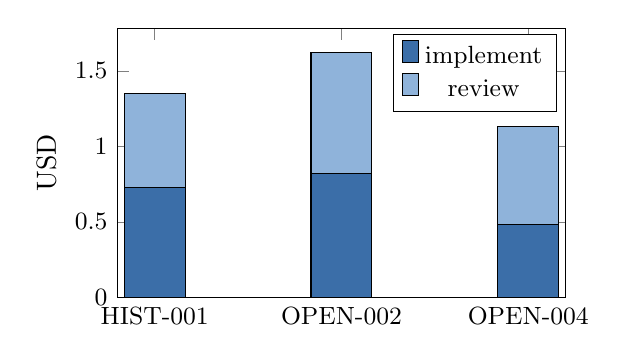
\begin{tikzpicture}
\begin{axis}[ybar stacked, bar width=22pt, width=0.6\linewidth, height=5cm,
  symbolic x coords={HIST-001,OPEN-002,OPEN-004},
  xtick=data, ylabel={USD}, ymin=0, legend style={at={(0.98,0.98)},anchor=north east,font=\small},
  tick label style={font=\small}]
\addplot[fill=impl] coordinates {(HIST-001,0.73) (OPEN-002,0.82) (OPEN-004,0.48)};
\addplot[fill=rev] coordinates {(HIST-001,0.62) (OPEN-002,0.80) (OPEN-004,0.65)};
\legend{implement, review}
\end{axis}
\end{tikzpicture}
\end{center}

\section*{Comparison with previous runs}

From \texttt{run-log.md}: the run that built these tickets cost \$25.44 for 10; this rework adds
\$4.10, so the PR's ten tickets cost \$29.54 (\$2.95 each). The previous session-review rework
of this lane (UI-004 and UI-005 on Opus, PR \#8) cost \$8.28 for two tickets.

\section*{Observations per model}

\begin{itemize}
  \item \textbf{gpt-6.1-sol xhigh, hard stage 2 (HIST-001, OPEN-002)}: red tests first through
        the real Main (result screen, review), then the smallest validation in
        \path{core/history.gd}; both show the corruption as a warning on the result screen.
  \item \textbf{gpt-6.1-sol high, stage 2 (OPEN-004)}: one regression through the real Main,
        Setup and Settings, then the re-check after the \texttt{await}; 7~min.
  \item \textbf{gpt-6.1-sol xhigh, review}: three approvals, no code in review (no round-0
        rows).
\end{itemize}

\section*{Driver and runtime issues}

None. The reopen kept earlier \texttt{Verdict: Reopen} lines unquoted so the driver counted
HIST-001's two reopens and gave it the hard implementer; every other line of the closed
records was quoted so the driver read no stale receipt or verdict.

\section*{Recommendations}

\begin{enumerate}
  \item Ticket reviews of persistence code should load a hand-edited file (a missing key, a
        wrong type) before approving. All three findings of this session review would have
        been caught that way or by changing a setting during an \texttt{await}.
  \item Keep the gpt-6.1-sol lineup: scoreboard row \texttt{gpt-6.1-sol high} $\rightarrow$
        \texttt{gpt-6.1-sol xhigh} 105 reviews, 17\% reopened, S2 rate 16\%.
\end{enumerate}

\section*{Human debt and proxy decisions}

No \texttt{Débito humano:} lines and no new \texttt{Proxy decided} lines in this rework; the
three tickets' earlier proxy decisions (listed in the previous report) stand unchanged.

\section*{Reopen attribution}

Session-review discoveries, recorded with \texttt{Discovery: session-review} and
\texttt{Round: -}; they do not enter the reopen rate. Judged by the foreman (Opus); the
reviewers are \texttt{gpt-6.1-sol}.

{\small
\noindent\begin{tabularx}{\linewidth}{@{}lXp{2.4cm}X@{}}
\toprule
Ticket & Finding & Label & Why \\
\midrule
HIST-001 & Partial or scalar result record in \path{stats.cfg}: script error, no warning & S2-explícito/\allowbreak código & Criteria 3 and 5. Review miss: yes. \\
OPEN-002 & Non-integer practice count: script error in target selection & S2-implícito & No criterion names corrupt input; failure path of its own persistence. Review miss: yes. \\
OPEN-004 & Checking enabled during the catalog load skips the required load check & S2-explícito/\allowbreak código & Criterion 2. Review miss: yes. \\
\bottomrule
\end{tabularx}
}

\section*{Scoreboard}

Same method as the previous report (lane clone for P-Chess, other repos' main checkouts). Rows
that moved: \texttt{gpt-6.1-sol high} $\rightarrow$ \texttt{gpt-6.1-sol xhigh} 102
$\rightarrow$ 105 reviews, 16 $\rightarrow$ 18 reopened (17\%), S2 rate 16\%;
\texttt{gpt-6.1-sol xhigh} $\rightarrow$ \texttt{gpt-6.1-sol xhigh} 4 $\rightarrow$ 10 reviews,
2 reopened (20\%, an anecdote); session-review discoveries 13 $\rightarrow$ 26 across repos (3
here, the rest EasyMath's), 20 of 22 known were earlier review misses; routine approvals 14
$\rightarrow$ 17.

\section*{Pending for the human}

\begin{enumerate}
  \item Re-review and merge PR \#10 (the supervising session runs the re-review).
  \item The manual checks and stage-1 triage listed in the previous report are unchanged.
\end{enumerate}

\end{document}
